% Author: Vitaly Parnas
\documentclass{article}

\usepackage{tikz}
% \usepackage[legalpaper, landscape, margin=2in]{geometry}
\usepackage[paperheight=15in,paperwidth=15in,margin=1in,heightrounded]{geometry}
\usepackage{amsmath}
\usetikzlibrary{mindmap,trees}
\usepackage{verbatim}
\graphicspath{ {images/} }

\begin{document}
\pagestyle{empty}

\begin{comment}
:Title: Algorithms Mind Map
:Tags: Manual, Mindmap

| Author: Vitaly Parnas
| Source: Algorithms Georgia Tech and MIT OCW Course Material

\end{comment}

\begin{tikzpicture}[mindmap, grow cyclic, every node/.style=concept,
    concept color=black,text=white,
    level 1/.append style={font=\Large\bfseries,level distance=8cm,sibling angle=72},
    level 2/.append style={font=\small\bfseries,level distance=4cm,sibling angle=45},
    level 3/.append style ={font=\tiny\bfseries},
    nucleus/.style= {concept, font=\huge\bfseries},
    ]

    % mbox content remains on one line
    \node [nucleus] {
\includegraphics[width=3cm,height=3cm,keepaspectratio]{algorithm_book}}
    child[concept color=blue!40!white,text=black,level distance=6cm] { node {Data \mbox{Structures}\\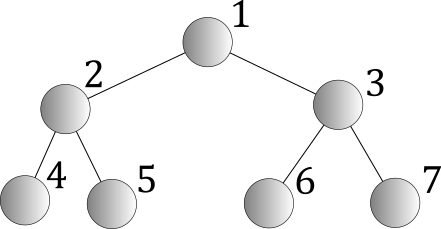
\includegraphics[width=2.5cm,height=2.5cm,keepaspectratio]{heap}}
        child{ node {Hashing} }
        child{ node {Priority Queue} 
            child{ node {Heap} }
            child{ node {Fibonacci Heap} }
        }
        child{ node {Graph} 
            child{ node {Adjacency List} }
            child{ node {Adjacency Matrix} }
            child{ node {Directed} }
            child{ node {Weighted} }
        }
        child{ node {Tree} }
    }
    child[concept color=red!70!white,text=black,level distance=7cm] { node {Sorting}
        child[sibling angle=72]{ node {Comparison $\Omega(n\log n)$} 
            child { node {Insertion} }
            child { node {Merge} }
            child { node {Bubble} }
            child { node {Selection} }
            child { node {Quicksort} }
            child { node {Heapsort} }
        }
        child{ node {Linear Time $\Omega(n)$} 
            child { node {Counting} }
            child { node {Radix} }
            child { node {Bucket} }
            child{ node {Order \mbox{Statistics}} 
                child { node {Median} }
                child { node {K-th \mbox{smallest}} }
            }
        }
    }
    child[concept color=green!50!white,text=black,level distance=6cm] { node {Analysis $\Theta,O,o$\\$\Omega,\omega$}
        child{ node {Amortized} 
            child { node {Potential Method} 
                child { node {Potential Func $\Phi(D)$}}
                child { node {Potential Diff $\Delta\Phi$}}
                child { node {Actual Cost $c$}}
                child { node {Amortized Cost $\hat{c}$}}
            }
        }
        child{ node {Probabilistic} 
            child { node {Randomized} 
                child { node {Monte-Carlo}}
                child { node {Las-Vegas}}
                child { node {Polynomial \mbox{Identities}}}
                child { node {Min-Cut}}
            }
            child { node {Hiring Problem}}
            child { node {Theory} 
                child { node {Expectation}}
                child { node {Random Vars}}
                child { node {Indep}}
            }
        }
        child{ node {Recursive} 
            child { node {Recurrence Tree} }
            child { node {Master Method} }
            child { node {Substitution} }
            child { node {Akra-Bazzi} }
        }
        child{ node {Proof} 
            child { node {Loop \mbox{Invariant}}}
            child { node {Inductive}}
            child { node {Constructive}}
            child { node {Contradiction}}
        }
    }
    child[concept color=red!30!white,text=black] { node {Design}
        child{ node {Divide and Conquer} 
            child { node {Matrix \mbox{Multiply}} 
                child { node {Standard} }
                child { node {Strassen} }
            }
            child { node {VLSI Layout} }
            child { node {Integer \mbox{Multiply}} }
            child { node {Max \mbox{Subarray}} }
        }
        child{ node {Dynamic Prog} 
            child { node {Recursive \mbox{Subproblem}} }
            child { node {Reuse \mbox{Calculations}} }
            child { node {Iterative Solution} }
        }
        child{ node {Greedy Alg} 
            child[sibling angle=72] { node {Optimal Solution} 
                child[sibling angle=72] { node {Greedy Choice} }
                child { node {Optimal \mbox{Substructure}} }
            }
            child { node {Matroid \mbox{$M = (S, \mathcal{I})$}} 
                child { node {Non-empty} }
                child { node {Hereditary} }
                child { node {Exchange \mbox{Property}} }
            }
        }
    }
    child[concept color=yellow!75!black,text=black] { node {Graph\\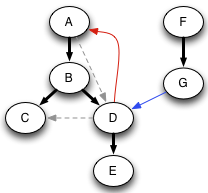
\includegraphics[width=2.5cm,height=2.5cm,keepaspectratio]{graph}}
        %child{ node {APSP} }
        child{ node {SSSP} 
            child { node {Bellman-Ford} 
                child { node {Negative Weights} }
            }
            child { node {Dijkstra's} 
                child { node {Non-zero weights} }
                child { node {Min \mbox{Priority} Q} }
            }
            child { node {LP \mbox{Feasibility}} 
                child { node {Diff \mbox{Constraints}} }
                child { node {Constraint Graph} }
            }
        }
        child{ node {MST} 
            child { node {Kruskal's} 
                child { node {Growing Forest} }
            }
            child { node {DAG} }
            child { node {Prim's} 
                child { node {Growing Tree} }
            }
        }
        child{ node {Search} 
            child { node {DFS} 
                child { node {Topological Sort} }
                child { node {Edges} 
                    child { node {Tree} }
                    child { node {Back} }
                    child { node {Forward} }
                    child { node {Cross} }
                }
                child { node {SCC} }
            }
            child { node {BFS} }
        }
        child[level distance=5cm]{ node {Max Flow} 
            child { node {Augmentation} }
            child { node {Properties} 
                child { node {Source} }
                child { node {Sink} }
                child { node {Capacity} }
                child { node {Residual Graph} }
                child { node {Cut} }
            }
            child { node {MF-\mbox{Min-Cut}} }
            child { node {Algorithms} 
                child { node {Ford \mbox{Folkerson}} }
                child { node {Scaling} }
                child { node {Edmonds-Karp} }
                child { node {Dinic's} }
            }
        }
    }
    ;
\end{tikzpicture}
\end{document}
